\documentclass[12pt]{article}
\usepackage[a4paper,margin=1in]{geometry}
\usepackage{ctex}
\usepackage{hyperref}
\usepackage[nameinlink,noabbrev]{cleveref}
\usepackage{booktabs}
\usepackage{longtable}
\usepackage{tabularx}
\usepackage{array}
\usepackage{xcolor}
\usepackage{enumitem}
\usepackage{listings}
\usepackage{tikz}
\usepackage{tcolorbox}
\usepackage{titlesec}
\usepackage{fancyhdr}
\usepackage{setspace}
\usepackage{caption}

\usetikzlibrary{positioning,arrows.meta,shapes.geometric,fit}
\tcbuselibrary{breakable,skins}

\hypersetup{
  colorlinks=true,
  linkcolor=blue!60!black,
  urlcolor=blue!60!black,
  pdftitle={Agentic Deep Research System 面试笔记},
  pdfauthor={Codex}
}

\setstretch{1.15}
\setlength{\parskip}{0.4em}
\setlength{\parindent}{2em}
\setlength{\headheight}{15pt}
\setlength{\emergencystretch}{2em}

\definecolor{codebg}{RGB}{248,248,248}
\definecolor{darkblue}{RGB}{18,58,98}
\definecolor{accent}{RGB}{0,98,155}
\definecolor{warn}{RGB}{176,69,0}
\definecolor{okgreen}{RGB}{19,110,62}

\lstdefinestyle{deepintel}{
  backgroundcolor=\color{codebg},
  basicstyle=\ttfamily\small,
  breaklines=true,
  columns=fullflexible,
  frame=single,
  framerule=0.3pt,
  keywordstyle=\color{darkblue}\bfseries,
  commentstyle=\color{okgreen},
  stringstyle=\color{warn},
  showstringspaces=false,
  tabsize=2,
  xleftmargin=0.5em,
  xrightmargin=0.5em
}
\lstset{style=deepintel}

\newtcolorbox{qaBox}[1]{
  breakable,
  colback=blue!2!white,
  colframe=accent!70!black,
  title=#1,
  fonttitle=\bfseries,
  arc=1mm
}

\newtcolorbox{riskBox}[1]{
  breakable,
  colback=orange!4!white,
  colframe=warn!80!black,
  title=#1,
  fonttitle=\bfseries,
  arc=1mm
}

\newtcolorbox{summaryBox}[1]{
  breakable,
  colback=gray!4!white,
  colframe=black!45,
  title=#1,
  fonttitle=\bfseries,
  arc=1mm
}

\titleformat{\section}{\Large\bfseries\color{darkblue}}{\thesection}{0.6em}{}
\titleformat{\subsection}{\large\bfseries\color{darkblue}}{\thesubsection}{0.6em}{}
\titleformat{\subsubsection}{\normalsize\bfseries\color{darkblue}}{\thesubsubsection}{0.6em}{}

\pagestyle{fancy}
\fancyhf{}
\fancyhead[L]{Agentic Deep Research System}
\fancyhead[R]{面试笔记}
\fancyfoot[C]{\thepage}

\newcommand{\term}[1]{\texttt{#1}}
\newcommand{\deepstrong}[1]{\textbf{#1}}


\begin{document}

\begin{titlepage}
  \centering
  \vspace*{3cm}
  {\Huge\bfseries Agentic Deep Research System\par}
  \vspace{0.8cm}
  {\LARGE 面试技术拷打笔记（TeX 正式版）\par}
  \vspace{1.2cm}
  {\large 面向：技术面试 / 架构深挖 / 治理闭环追问 / 高压交叉盘问\par}
  \vfill
  {\large 版本：v2.0\par}
  {\large 日期：2026-05-27\par}
\end{titlepage}

\tableofcontents
\newpage

\section{怎么使用这份笔记}

\begin{summaryBox}{这份文档不是项目报告}
这份文档的用途不是把项目按模块介绍一遍，而是训练一种更适合技术面试的表达方式：面试官会先确认你是不是自己做过，再追问你为什么这么选，接着看你能不能把边界、缺陷、治理和演进路线讲清楚。
\end{summaryBox}

\begin{qaBox}{建议的回答顺序}
回答时不要一上来就堆框架名。最稳的顺序是：先定义系统解决什么问题，再讲主链路怎么跑，再讲为什么这么选，再讲当前已经做到哪里，最后讲哪些地方还没做完、准备怎么补。这样既像工程师，也不像背稿。
\end{qaBox}

\begin{riskBox}{这份笔记的使用原则}
第一，不要把设计稿说成已上线功能。第二，不要把历史 bug 说成当前仍存在的问题。第三，不要把治理愿景说成生产级闭环。第四，遇到面试官追问时，优先讲事实、边界和取舍，不要用空话兜底。
\end{riskBox}

\section{第一轮拷打：先把项目说清楚}

\begin{summaryBox}{这一轮面试官在试什么}
这一轮不是考你会不会背名词，而是在判断你能不能用两到三分钟把系统定义准确。面试官真正想听的是：这到底是不是一个严肃的研究型系统，还是只是把搜索、RAG 和报告拼到一起的 Demo。
\end{summaryBox}

\subsection{先用一句话定义这个项目}
\begin{qaBox}{一句话总述}
这是一个以 LangGraph 为业务编排内核、以 Search / Browser / RAG 为取证能力、以 Analyst / Reflection / Report 为分析闭环、并逐步向治理型 Agent 演进的研究系统。
\end{qaBox}

\subsection{面试开场应该怎么讲}
\begin{summaryBox}{推荐开场}
如果面试官先问“这个系统是干什么的”，最稳的讲法不是直接说“这是一个 AI Agent”，而是先把它定义成一个 \term{evidence-driven deep research workflow}。它的核心目标不是闲聊，不是通用办公自动化，而是围绕“搜索、取证、对比、分析、引用、报告”构造一条可重复执行的研究链路。
\end{summaryBox}

我通常会用下面这段话开场：

\begin{qaBox}{标准开场答案}
这个系统的目标是把用户问题转换成一张可执行研究图。Planner 先把问题拆成 DAG，Search / Browser / RAG 节点分别去互联网、网页和内部知识库取证，Analyst 负责综合证据形成结构化分析，Reflection 负责做事实、一致性和引用覆盖率校验，最后 Report 输出带引用的研究报告。系统的设计重点不是单次回答得多花哨，而是证据链、失败语义、预算控制和后续治理扩展能力。
\end{qaBox}

\subsection{系统的分层怎么看}
\begin{itemize}[leftmargin=2em]
  \item 编排层：LangGraph StateGraph，负责节点、条件边、循环和并行。
  \item 能力层：Planner / Search / Browser / RAG / Analyst / Reflection / Report。
  \item 状态层：ResearchState、DAG、checkpoint、trace、tool audit、budget state。
  \item 数据层：PostgreSQL + pgvector，存文档、session、citation、tool audit、budget state。
  \item 交互层：FastAPI + SSE，负责创建任务、查询状态、流式推送进度。
  \item 治理层：guardrail、runtime status、budget breaker、approval source of truth、未来 Harness supervisor 与 MCP proxy。
\end{itemize}

\subsection{为什么这个系统不是简单的 RAG 问答}
\begin{qaBox}{核心差异}
RAG 问答通常是“检索一轮，再回答一轮”。这个系统做的是“先规划，再多源取证，再综合分析，再反思校验，再决定是否重规划”。它把单次回答升级成了一条带状态、带条件分支、带恢复与治理约束的研究流水线。
\end{qaBox}

\section{第二轮拷打：为什么这么选，而不是别的}

\begin{summaryBox}{这一轮面试官在试什么}
当你把系统讲清楚之后，面试官通常会立刻追问选型理由。这里最怕两种答法：一种是“社区都这么用”，另一种是“我觉得这个更先进”。正确答法必须同时包含备选方案、比较维度和最终取舍。
\end{summaryBox}

\begin{riskBox}{这一轮最容易翻车的地方}
不要把“能用”讲成“唯一正确”。也不要回避被否选方案，因为真正做过工程的人一定经历过权衡，而不是从一开始就知道唯一答案。
\end{riskBox}

\subsection{Agent 编排框架：为什么选择 LangGraph}
\begin{qaBox}{结论}
研究任务本质上不是线性 \term{Chain}，而是带并行、条件分支和重规划循环的状态机，所以选择 LangGraph，而不是只用 LangChain 的串联式抽象。
\end{qaBox}

\begin{center}
\small
\begin{tabularx}{\textwidth}{>{\bfseries}lXXXX}
\toprule
维度 & LangGraph & LangChain & AutoGen & CrewAI \\
\midrule
核心抽象 & 状态机 / 图编排 & 链和工具集成层 & 对话式多 Agent & 角色协作脚本 \\
并行与 fan-out & 原生 \term{Send API} & 需手动拼接 & 可做但偏消息流 & 较弱 \\
条件边 & 强 & 中 & 中 & 弱 \\
循环与重规划 & 强 & 弱 & 中 & 弱 \\
检查点恢复 & 支持 & 有限 & 有限 & 弱 \\
适合研究 DAG & 很适合 & 一般 & 偏实验 & 偏演示 \\
\bottomrule
\end{tabularx}
\end{center}

\begin{summaryBox}{选择理由}
这里至少有两个可行方案。方案 A 是继续用 LangChain，把 Planner、Search、Report 串起来，再自己维护一套 if-else。优点是简单，缺点是并行、循环、恢复都会越来越别扭。方案 B 是直接把研究流程建模成一张图，让节点、边、状态、路由都显式化。最终选择 LangGraph，就是选择方案 B。
\end{summaryBox}

\begin{qaBox}{面试回答模板}
LangGraph 解决的是“复杂多步骤任务如何以显式状态机方式执行”。研究型任务天然需要 DAG、并行、条件边和循环重规划，这四点是 LangGraph 的强项。LangChain 很适合做工具和模型的胶水层，但不适合单独承担复杂业务工作流编排。
\end{qaBox}

\subsection{LangGraph 和 DAG 的关系}
\begin{qaBox}{追问答案}
DAG 是业务层面的研究计划图，StateGraph 是执行层面的工作流图。Planner 生成的 DAG 解决“研究步骤怎么拆”，LangGraph StateGraph 解决“这些步骤怎样被调度、聚合、校验、循环和恢复”。DAG 是数据，StateGraph 是执行器。
\end{qaBox}

\subsection{为什么还要 Harness，而不是只靠 LangGraph}
\begin{center}
\small
\begin{tabularx}{\textwidth}{>{\bfseries}lXXX}
\toprule
方案 & 做法 & 优点 & 缺点 \\
\midrule
方案 A & 生命周期、重试、审批、恢复都塞进 LangGraph & 单层编排、概念简单 & 图会越来越重，治理逻辑和业务逻辑耦合 \\
方案 B & LangGraph 管业务图，Harness 管 supervisor & 治理边界清晰，适合长任务 & 多一层状态同步与恢复控制 \\
\bottomrule
\end{tabularx}
\end{center}

\begin{qaBox}{最终选择}
当前项目的长期正确方向是方案 B：LangGraph 负责业务编排，Harness 负责任务级控制面。因为你真正要治理的是“失败后怎么恢复、预算超了怎么刹车、审批后怎么恢复、worker 怎么抢租约”，这些都不是业务 DAG 最擅长表达的东西。
\end{qaBox}

\subsection{LLM 选型：为什么强调结构化输出和工具调用}
\begin{summaryBox}{选型标准}
这个系统里的模型不是单纯负责写文案，它要做 DAG 生成、JSON 结构化输出、事实校验、引用覆盖率分析和报告生成，所以第一优先级不是“最会聊天”，而是“最稳定地产生结构化结果”。
\end{summaryBox}

\begin{center}
\small
\begin{tabularx}{\textwidth}{>{\bfseries}lXXX}
\toprule
维度 & 倾向项 & 原因 & 对本项目的影响 \\
\midrule
工具调用稳定性 & 高优先级 & Planner / Reflection 都依赖结构化结果 & 降低解析失败和 fallback 频率 \\
中文能力 & 高优先级 & 用户查询、网页、报告以中文为主 & 减少跨语言语义损耗 \\
成本 & 高优先级 & 深研究任务 token 消耗天然高 & 决定是否能高频运行 \\
通用推理上限 & 中优先级 & 重要，但不是唯一约束 & 可由反思、检索和多轮流程补强 \\
\bottomrule
\end{tabularx}
\end{center}

\begin{qaBox}{面试时的稳妥表述}
我对模型选型的原则不是盲目追逐最强模型，而是优先看三个维度：结构化输出是否稳定、工具调用是否稳定、中文与成本是否平衡。因为在研究型 Agent 里，模型失败往往不是“文风不够好”，而是 JSON 不可解析、校验结果不稳定、成本高到没法长期运行。
\end{qaBox}

\subsection{浏览器自动化：为什么选择 Playwright}
\begin{center}
\small
\begin{tabularx}{\textwidth}{>{\bfseries}lXXXX}
\toprule
维度 & Playwright & Puppeteer & Selenium & 结论 \\
\midrule
异步模型 & 原生 async & 原生 async & 传统同步为主 & Playwright 更适合 Python async 服务 \\
自动等待 & 强 & 中 & 弱 & 减少页面交互竞态 \\
多浏览器支持 & Chromium/FF/WebKit & 偏 Chromium & 强 & Playwright 更平衡 \\
工程稳定性 & 高 & 中 & 中 & 对研究型抓取更合适 \\
\bottomrule
\end{tabularx}
\end{center}

\begin{qaBox}{核心回答}
我选 Playwright 的原因不是“它比较新”，而是它更贴合 Browser Use 场景。研究型浏览器节点经常面对动态加载、延迟渲染、滚动加载和反检测问题，Playwright 的自动等待、页面生命周期控制和无头执行能力更容易形成稳定工程实现。
\end{qaBox}

\subsection{为什么要实现三层浏览器提取策略}
\begin{qaBox}{设计理由}
不是所有页面都值得深度提取。浏览器节点如果默认把整页内容吃满，会直接推高 token 消耗、拉长时延、放大噪音。所以设计成 \term{snippet / skim / deep} 三层提取，本质上是把内容质量和成本一起治理。
\end{qaBox}

\begin{itemize}[leftmargin=2em]
  \item \term{snippet}：优先抓 meta 和少量核心文本，适合快速判断页面是否有价值。
  \item \term{skim}：抓主要段落，适合普通文章和资讯。
  \item \term{deep}：抓更多标题、段落、列表、结构化片段，适合权威报告和高价值页面。
\end{itemize}

\subsection{RAG 与向量库：为什么选择 pgvector}
\begin{center}
\small
\begin{tabularx}{\textwidth}{>{\bfseries}lXXXX}
\toprule
维度 & pgvector & Qdrant & Chroma & Pinecone \\
\midrule
部署复杂度 & 低 & 中 & 低 & SaaS \\
事务一致性 & 强 & 弱 & 弱 & 弱 \\
和业务表 JOIN & 方便 & 较弱 & 较弱 & 不方便 \\
全文搜索协同 & 强 & 需外部系统 & 弱 & 需外部系统 \\
运维成本 & 低 & 中 & 低 & 高 \\
\bottomrule
\end{tabularx}
\end{center}

\begin{qaBox}{最终选择}
我选 pgvector，不是因为它在纯向量召回上一定最强，而是因为它对这个项目的整体工程复杂度最低。文档、元数据、citation、research session、全文索引和向量索引都在同一套 PostgreSQL 里，事务一致性和数据联查能力非常强。
\end{qaBox}

\subsection{为什么内部检索不是“查一下就回答”}
\begin{qaBox}{核心区分}
内部 RAG 在这个系统里不是回答器，而是证据源。它负责给出可引用片段、提供内部知识背景、帮助决定是否还要联网搜索，但最终回答仍然要经过 Analyst、Reflection 和 Report 链路。
\end{qaBox}

\section{第三轮拷打：系统到底怎么跑，状态怎么流}

\begin{summaryBox}{这一轮面试官在试什么}
这一轮会从“你为什么这样设计”切到“这个系统运行时到底发生了什么”。如果你只能讲模块名，讲不清状态怎么变化、节点怎么路由、失败怎么传播，面试官会判断你更像读过代码，而不是做过系统。
\end{summaryBox}

\subsection{从 API 到报告的完整生命周期}
\begin{center}
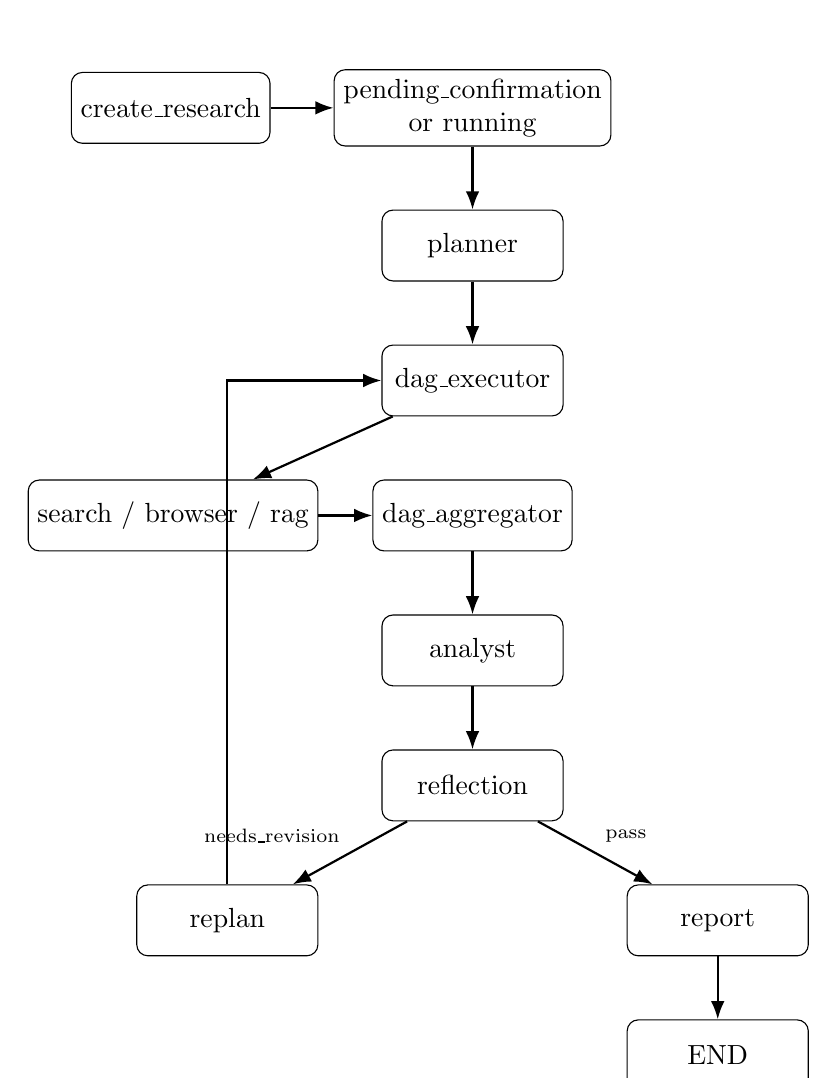
\begin{tikzpicture}[
  node distance=8mm and 8mm,
  box/.style={draw, rounded corners, align=center, minimum width=23mm, minimum height=9mm},
  flow/.style={-Latex, thick}
]
\node[box] (create) {create\_research};
\node[box, right=of create] (pending) {pending\_confirmation\\or running};
\node[box, below=of pending] (planner) {planner};
\node[box, below=of planner] (dagx) {dag\_executor};
\node[box, below left=of dagx] (tools) {search / browser / rag};
\node[box, below=of dagx] (agg) {dag\_aggregator};
\node[box, below=of agg] (analyst) {analyst};
\node[box, below=of analyst] (reflection) {reflection};
\node[box, below left=of reflection] (replan) {replan};
\node[box, below right=of reflection] (report) {report};
\node[box, below=of report] (end) {END};

\draw[flow] (create) -- (pending);
\draw[flow] (pending) -- (planner);
\draw[flow] (planner) -- (dagx);
\draw[flow] (dagx) -- (tools);
\draw[flow] (tools) -- (agg);
\draw[flow] (agg) -- (analyst);
\draw[flow] (analyst) -- (reflection);
\draw[flow] (reflection) -- node[above left, font=\scriptsize]{needs\_revision} (replan);
\draw[flow] (replan) |- (dagx);
\draw[flow] (reflection) -- node[above right, font=\scriptsize]{pass} (report);
\draw[flow] (report) -- (end);
\end{tikzpicture}

\end{center}

\begin{summaryBox}{现状说明}
当前生命周期是：\term{create\_research} 建 session，状态先进入 \term{pending\_confirmation} 或 \term{running}，随后后台运行 LangGraph：\term{planner -> dag\_executor -> search/browser/rag -> dag\_aggregator -> analyst -> reflection -> replan/report -> END}。这条主链路已经打通，是系统最核心的业务骨架。
\end{summaryBox}

\subsection{公开状态与内部运行状态为什么要分开}
\begin{qaBox}{核心设计}
对外 API 的状态要稳定，对内运行状态要足够细。公开层只需要 \term{pending / running / completed / failed} 这种粗粒度语义，但治理层必须区分 \term{awaiting\_approval / retryable\_failed / terminal\_failed / completed}，否则失败恢复、审批暂停和预算熔断都没法精确表达。
\end{qaBox}

\subsection{ResearchState 为什么是这个系统的核心}
\begin{lstlisting}[language=Python,caption={ResearchState 中最关键的状态维度}]
task_id / user_query / status / session
dag / current_executing_nodes / completed_nodes
tool_histories / node_outcomes / collected_evidence
verification / revision_needed / revision_count
runtime_status / budget_state / pending_approvals
agent_trace / guardrail_trace / errors
\end{lstlisting}

\begin{summaryBox}{设计原则}
ResearchState 不是简单的“共享上下文容器”，而是整个工作流的单一运行时状态机载体。凡是会影响路由、恢复、预算、审批和审计的字段，都应该显式出现在 state 里，而不是藏在零散的局部变量中。
\end{summaryBox}

\subsection{Planner 如何生成 DAG，为什么还需要 fallback}
\begin{qaBox}{面试回答}
Planner 的职责不是直接给最终答案，而是把用户问题拆成一张可执行研究图。它会让 LLM 生成 \term{DAGDefinition}，里面包含节点类型、查询内容、依赖关系和并行性。但因为 LLM 可能输出坏 JSON、空结果或不合理节点，所以必须准备 fallback DAG，保证流程至少能退化成“搜索 + 浏览 + 内部检索 + 分析”这条保底路径。
\end{qaBox}

\subsection{DAG 的正确性如何保证}
\begin{itemize}[leftmargin=2em]
  \item 数据结构层：Planner 输出被解析成 \term{PlanNode / PlanEdge / DAGDefinition}。
  \item 执行层：\term{get\_executable\_order()} 用拓扑思路分批求可执行节点。
  \item 容错层：非法节点会被过滤，Planner 失败时回退到 fallback DAG。
  \item 策略层：系统还会强制内部 RAG 先于 Web 节点执行，形成 internal-first 检索策略。
\end{itemize}

\subsection{为什么要先 internal RAG，再决定要不要联网}
\begin{qaBox}{设计理由}
研究型系统不应该把互联网搜索当作唯一真相源。内部知识库通常更贴近企业语境，也更可控，所以系统会优先执行内部 RAG，再根据命中情况和策略判断是否继续走 Web。这样既减少无意义联网，也能降低把内部问题完全外部化的风险。
\end{qaBox}

\subsection{工具节点为什么必须返回显式结果契约}
\begin{lstlisting}[language=Python,caption={NodeOutcome 契约}]
NodeOutcome = TypedDict("NodeOutcome", {
    "node_id": str,
    "tool_call_id": str | None,
    "tool_name": str,
    "status": Literal[
        "success",
        "retryable_error",
        "terminal_error",
        "awaiting_approval",
        "skipped",
    ],
    "error_category": str | None,
    "error_message": str | None,
    "retry_count": int,
    "tokens_used": int,
    "cost_usd": float,
    "result_count": int,
    "approval_request_id": str | None,
})
\end{lstlisting}

\begin{qaBox}{为什么不能只靠 tool\_histories}
\term{tool\_histories} 更适合审计，不适合做唯一状态源。因为审计记录的目标是“发生了什么”，而路由的目标是“下一步怎么办”。如果失败语义只藏在 tool history 里，聚合器很容易在语义不明确时把节点误标成完成。显式的 \term{NodeOutcome} 正是为了解决这个问题。
\end{qaBox}

\subsection{Search / Browser / RAG 三类节点如何分工}
\begin{itemize}[leftmargin=2em]
  \item Search：适合快速事实、数据、新闻入口、网址发现。
  \item Browser：适合深读文章、结构化页面提取、动态网页。
  \item RAG：适合内部资料、历史文档、背景知识和企业语义上下文。
\end{itemize}

\begin{summaryBox}{面试回答模板}
这三类节点不是冗余，而是故意分层。Search 负责广撒网，Browser 负责深挖高价值页面，RAG 负责内部可控证据。真正有价值的研究系统不是任何问题都扔给浏览器，而是先判断哪种证据源最值得花成本。
\end{summaryBox}

\section{第四轮拷打：关键机制是不是你真的做过}

\begin{summaryBox}{这一轮面试官在试什么}
这一轮会专门挑几个最容易暴露“只懂概念、不懂实现”的点来问，例如 Reflection 有什么用、RRF 为什么合理、Checkpointer 到底帮你解决了什么。这里需要把抽象概念落回具体执行语义。
\end{summaryBox}

\subsection{Analyst 为什么单独存在}
\begin{qaBox}{核心作用}
Analyst 的意义是把多源证据从“片段集合”转成“结构化分析”。Search、Browser、RAG 拿回来的是证据，Analyst 负责做事实归类、冲突识别、分析组织和初步结论形成。
\end{qaBox}

\subsection{Reflection 为什么不能省掉}
\begin{qaBox}{核心回答}
如果没有 Reflection，整个系统就会退化成“拿到一些证据后直接写报告”。Reflection 的职责是把回答质量结构化成 \term{overall\_confidence}、\term{citation\_coverage}、\term{needs\_revision} 等信号，再由图路由决定是否重规划。它不是装饰，而是把“能不能继续往前走”显式化。
\end{qaBox}

\subsection{Reflection 和传统 reviewer 的区别}
\begin{itemize}[leftmargin=2em]
  \item Reviewer 更偏规则门禁或人工审查。
  \item Reflection 更偏模型辅助的自校验与质量评分。
  \item 在当前项目里，Reflection 已经存在，但更硬的动作审批 reviewer 还没有形成独立工作流分支。
\end{itemize}

\subsection{RRF 融合检索为什么合理}
\begin{lstlisting}[language=Python,caption={RRF 的直观公式}]
score(d) = sum(1 / (k + rank(d)))
\end{lstlisting}

\begin{summaryBox}{设计理由}
RRF 不是为了追求算法花哨，而是为了在多路检索结果之间取得稳定折中。向量相似度、关键词匹配、重排结果的分值尺度往往不一致，直接线性加权很脆弱；RRF 只依赖 rank，更稳、更简单，也更容易工程落地。
\end{summaryBox}

\subsection{Checkpointer 的真实价值是什么}
\begin{qaBox}{核心答案}
\term{thread\_id=session\_id} 保证的是会话隔离，Checkpointer 提供的是状态恢复能力。它能让 LangGraph 在节点边界保存执行快照，使流程在中断后有机会从已知状态继续。但要注意，检查点本身不是完整治理方案，它不自动解决预算、审批、审计和 supervisor 恢复控制。
\end{qaBox}

\subsection{为什么 SSE 对这个系统重要}
\begin{qaBox}{核心理由}
研究任务天然是长任务，如果没有流式可观测性，用户只能看到一个很长的 loading。SSE 的价值不是“酷炫实时输出”，而是把 agent trace、tool 进度、状态变化、报告片段和错误事件透明推给前端，让任务变成可感知、可追踪、可中断观察的过程。
\end{qaBox}

\section{第五轮拷打：性能、成本和资源怎么扛}

\begin{summaryBox}{这一轮面试官在试什么}
很多候选人在这里会只讲“做了并发、做了缓存、做了优化”。这不够。研究型 Agent 的资源问题至少包含三类：时延、token/cost、数据库与工具开销。面试官想看的是你有没有把它们视为同一个系统问题。
\end{summaryBox}

\subsection{为什么并行执行能显著降低时延}
\begin{lstlisting}[language=Python,caption={LangGraph Send API 的作用}]
dag_executor -> [Send("search"), Send("browser"), Send("rag")]
\end{lstlisting}

\begin{qaBox}{面试回答}
如果 Search、Browser、RAG 串行执行，总时延接近三者之和；并行 fan-out 后，总时延更接近三者中的最大值。这类任务的瓶颈往往在 I/O，而不是 CPU，所以并行调度的收益很高。
\end{qaBox}

\subsection{Token 优化策略}
\begin{itemize}[leftmargin=2em]
  \item 输出长度分 \term{short / medium / long} 三档，不只是影响报告 token，也同步影响搜索次数、RAG 返回量和 citation 上限。
  \item 浏览器内容用 \term{snippet / skim / deep} 控制页面读取粒度。
  \item RAG 侧采用候选召回 + 排序 + 截断，避免把低价值片段灌入上下文。
  \item 最终报告阶段再根据预算控制输出规模，避免前面省下来的 token 最后一次性烧光。
\end{itemize}

\subsection{数据库优化怎么看}
\begin{itemize}[leftmargin=2em]
  \item 文档层：向量索引承担 ANN，全文索引承担关键词检索。
  \item 业务层：research session、citation、tool audit、budget state 都在同一库里，降低同步复杂度。
  \item 可观测层：指标与 trace 可以按 session 维度做统计和聚合。
\end{itemize}

\section{第六轮拷打：你怎么证明它没胡来}

\begin{summaryBox}{这一轮面试官在试什么}
会做流程不等于会做系统。面试官在这一轮通常会问：你怎么知道它真的在工作，而不是表面有输出？你怎么定位问题？你怎么区分是模型错了、工具错了、还是治理规则拦住了？
\end{summaryBox}

\subsection{我会看哪些指标}
\begin{center}
\small
\begin{tabularx}{\textwidth}{>{\bfseries}lXX}
\toprule
维度 & 代表指标 & 作用 \\
\midrule
工作流层 & 成功率、P95 时长、重规划次数 & 看流程稳定性 \\
工具层 & tool success rate、平均时长、错误分类 & 看节点可靠性 \\
质量层 & citation coverage、overall confidence、hallucination rate & 看答案质量 \\
成本层 & used tokens、used cost、tool calls、wall clock & 看预算消耗 \\
治理层 & approval count、budget stop count、terminal failures & 看可控性 \\
\bottomrule
\end{tabularx}
\end{center}

\subsection{trace 为什么要分成几条线}
\begin{itemize}[leftmargin=2em]
  \item \term{agent\_trace}：高层流程事件，适合 UI 和时间线回放。
  \item \term{guardrail\_trace}：安全和路由决策，适合解释“为什么被拦”。
  \item \term{tool\_call\_audit}：单次工具调用明细，适合法证级追踪。
\end{itemize}

\begin{summaryBox}{设计观点}
把所有东西都塞进一条 trace 里，看起来简单，实际上后面既不好查，也不好给不同角色消费。高层事件、护栏决策、单次调用明细这三类数据天然就是不同层次，拆开才有意义。
\end{summaryBox}

\section{第七轮拷打：哪些能吹，哪些不能吹}

\begin{summaryBox}{这一轮面试官在试什么}
这轮最考验真实性。很多项目不是死在技术上，而是死在表述上。你如果把设计稿说成已经上线，或者把半成品说成生产级，懂行的面试官一追就穿。这里必须把“已做完”“已部分落地”“还在设计”分开讲。
\end{summaryBox}

\subsection{当前真实完成度应该怎么诚实表达}
\begin{riskBox}{建议表述}
当前系统已经具备研究主链路、DAG 编排、反思校验、SSE trace 和基本预算治理能力，但完整治理闭环仍在演进中。更准确的说法是：它已经是一个能工作的研究型 Agent 系统，但离严格意义上的生产级执行治理系统还有距离。
\end{riskBox}

\begin{center}
\small
\begin{tabularx}{\textwidth}{>{\bfseries}lXX}
\toprule
能力项 & 当前状态 & 面试表述建议 \\
\midrule
主任务生命周期 & 已打通 & 可以说“已实现主链路” \\
失败语义 & 已从历史 bug 修到显式 outcome & 可以说“失败语义已显式化” \\
工具审计 & 已有独立 \term{tool\_call\_audit} & 可以说“审计闭环已增强，但仍非 crash-safe” \\
会话级预算 breaker & 已有最小可用版 & 可以说“已支持硬熔断，但 token/cost 仍部分依赖估算” \\
动作级审批 & 仍未完成 & 不能说“动作级审批已上线” \\
Harness supervisor & 设计已定，代码未完整接入 & 不能说“已实现任务级恢复控制” \\
MCP 安全接入 & 设计已定，尚未真正接入 & 不能说“已安全支持 MCP” \\
\bottomrule
\end{tabularx}
\end{center}

\subsection{失败语义为什么是治理第一优先级}
\begin{center}
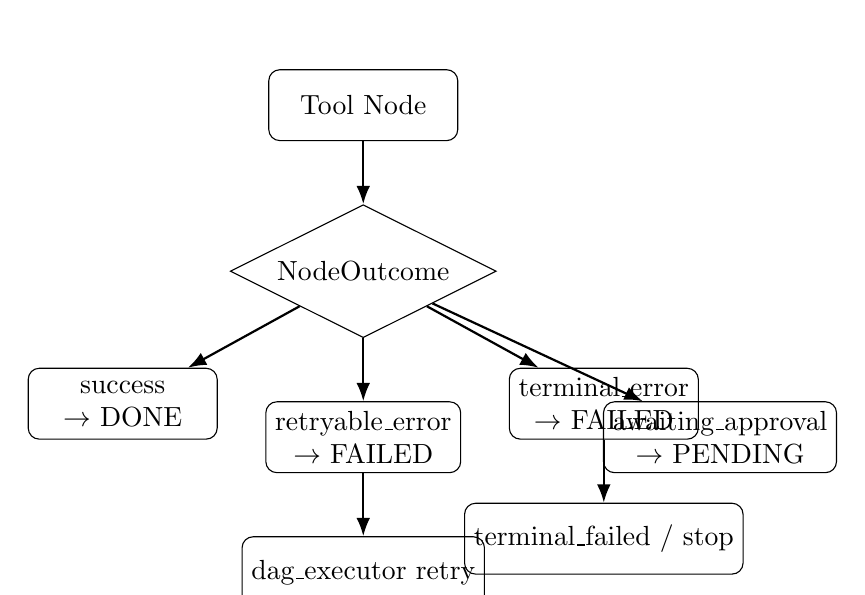
\begin{tikzpicture}[
  node distance=8mm and 10mm,
  box/.style={draw, rounded corners, align=center, minimum width=24mm, minimum height=9mm},
  decision/.style={diamond, draw, align=center, aspect=2},
  flow/.style={-Latex, thick}
]
\node[box] (tool) {Tool Node};
\node[decision, below=of tool] (outcome) {NodeOutcome};
\node[box, below left=of outcome] (success) {success\\$\rightarrow$ DONE};
\node[box, below=of outcome] (retry) {retryable\_error\\$\rightarrow$ FAILED};
\node[box, below right=of outcome] (terminal) {terminal\_error\\$\rightarrow$ FAILED};
\node[box, right=18mm of retry] (approval) {awaiting\_approval\\$\rightarrow$ PENDING};
\node[box, below=of retry] (executor) {dag\_executor retry};
\node[box, below=of terminal] (stop) {terminal\_failed / stop};

\draw[flow] (tool) -- (outcome);
\draw[flow] (outcome) -- (success);
\draw[flow] (outcome) -- (retry);
\draw[flow] (outcome) -- (terminal);
\draw[flow] (outcome) -- (approval);
\draw[flow] (retry) -- (executor);
\draw[flow] (terminal) -- (stop);
\end{tikzpicture}

\end{center}

\begin{summaryBox}{历史 bug 与当前状态}
这个系统历史上最关键的问题，是工具节点失败后聚合器可能仍然把节点当成完成。这个 bug 现在已经修掉了，工具节点通过 \term{NodeOutcome} 回传显式状态，聚合器按 \term{success / retryable\_error / terminal\_error / awaiting\_approval / skipped} 更新节点。它之所以值得在面试里重点讲，是因为它直接体现了“为什么失败语义必须显式建模”。
\end{summaryBox}

\subsection{会话级预算治理现在到了什么程度}
\begin{qaBox}{当前可说的事实}
当前项目已经不是只有长度档位了，图内已经接入最小可用的 \term{session-level budget breaker}，包括 \term{max\_tool\_calls}、\term{max\_wall\_clock\_seconds}，以及预留的 \term{max\_total\_tokens / max\_cost\_usd} 通道。达到硬阈值时，系统会跳过剩余工具节点，进入分析与部分报告，而不是继续无限烧。
\end{qaBox}

\begin{riskBox}{必须诚实说明的边界}
当前 token/cost 通道虽然已经接到 LLM usage 和 budget state，但仍不是完全精确计费系统。一方面部分模型返回 usage 需要估算，另一方面 tool 侧的 cost 仍不全，所以现阶段更可靠的是 \term{tool\_calls} 和 \term{wall\_clock} 维度的硬熔断。
\end{riskBox}

\subsection{法证级审计现在到了什么程度}
\begin{qaBox}{当前结论}
现在已经不只是 \term{tool\_histories} 运行时累积状态了，系统已新增独立的 \term{tool\_call\_audit} 表，把单次工具调用拆成独立记录。这样 session 结果查询和审计查询不再混在一行 JSON 里。
\end{qaBox}

\begin{riskBox}{仍未闭环的点}
目前工具审计和预算状态主要在 workflow 收尾时统一落库，因此还不是 crash-safe 的实时法证闭环。如果进程在中途崩掉，内存中尚未持久化的调用明细和预算中间态仍可能丢失。这正是下一步需要 Harness 和 batch boundary checkpoint 来补的位置。
\end{riskBox}

\section{第八轮拷打：邪恶 Agent 怎么管住}

\begin{summaryBox}{这一轮面试官在试什么}
这轮不是问“你会不会做 Agent”，而是问“你敢不敢把 Agent 放进真实系统”。如果面试官开始追问审批、预算、审计、MCP、恢复、权限边界，说明他在看你有没有治理视角，而不只是能力视角。
\end{summaryBox}

\subsection{治理闭环现状判断}
\begin{summaryBox}{一句话}
现在系统已经有 workflow、trace、tool audit、budget breaker 的基础闭环，但审批、恢复和外部工具信任边界还没有完全闭合。
\end{summaryBox}

\subsection{审批状态源（Approval Source of Truth）}
\begin{center}
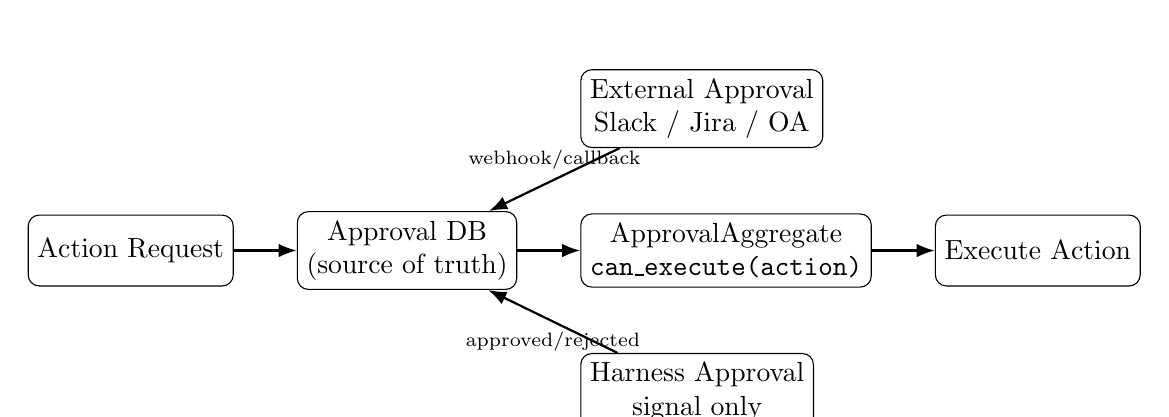
\begin{tikzpicture}[
  node distance=8mm and 8mm,
  box/.style={draw, rounded corners, align=center, minimum width=24mm, minimum height=9mm},
  flow/.style={-Latex, thick}
]
\node[box] (action) {Action Request};
\node[box, right=of action] (db) {Approval DB\\(source of truth)};
\node[box, above right=of db] (external) {External Approval\\Slack / Jira / OA};
\node[box, below right=of db] (harness) {Harness Approval\\signal only};
\node[box, right=of db] (aggregate) {ApprovalAggregate\\\term{can\_execute(action)}};
\node[box, right=of aggregate] (exec) {Execute Action};

\draw[flow] (action) -- (db);
\draw[flow] (external) -- node[above, font=\scriptsize]{webhook/callback} (db);
\draw[flow] (harness) -- node[below, font=\scriptsize]{approved/rejected} (db);
\draw[flow] (db) -- (aggregate);
\draw[flow] (aggregate) -- (exec);
\end{tikzpicture}

\end{center}

\begin{qaBox}{固定立场}
动作级审批的最终权威源必须是本地数据库审批单。Harness、Slack、Jira、ServiceNow 这类系统都可以作为审批信号源，但最终 \term{can\_execute(action)} 的判断必须由本地审批聚合根负责。
\end{qaBox}

\begin{center}
\small
\begin{tabularx}{\textwidth}{>{\bfseries}lXXX}
\toprule
来源 & 谁是权威 & 优点 & 问题 \\
\midrule
LOCAL DB & 系统自己 & 单一真相源、查询直观、审计强 & 工程量最大 \\
HARNESS & Harness 平台 & UI、RBAC、流程现成 & 易和业务状态漂移 \\
EXTERNAL & Slack/Jira/OA 等 & 贴合企业习惯 & 远端状态和本地状态同步复杂 \\
\bottomrule
\end{tabularx}
\end{center}

\begin{lstlisting}[caption={ApprovalAggregate 的建议最小字段}]
approval_id
action_id
approval_source
external_id
status
version
approved_by
expire_time
\end{lstlisting}

\subsection{为什么外部审批只能是信号，不能是唯一裁决}
\begin{qaBox}{原因}
因为只要允许多个 source of truth 并存，就一定会遇到状态漂移：例如 Harness 已经批了，但 DB 仍是 pending；或者 Slack 上已经通过，但 agent 因为没看到本地状态变化再次发起执行。真正要避免的不是“查不到谁批了”，而是“重复执行危险动作”。
\end{qaBox}

\subsection{Harness 外挂设计}
\begin{center}
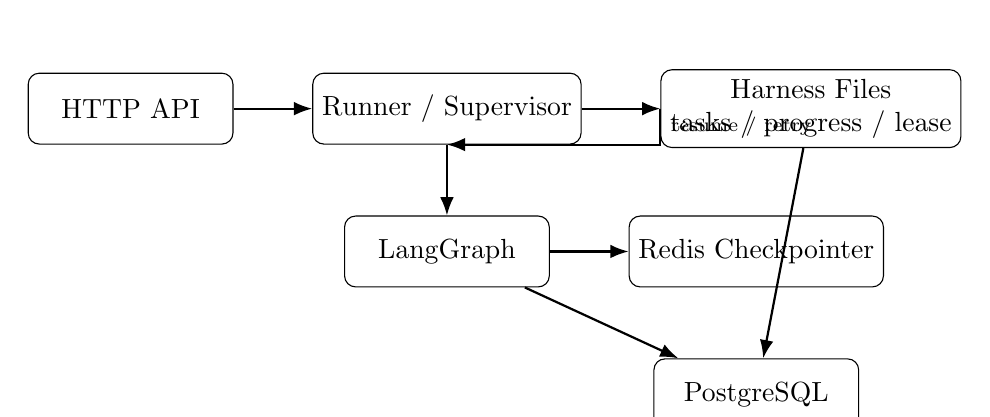
\begin{tikzpicture}[
  node distance=9mm and 10mm,
  box/.style={draw, rounded corners, align=center, minimum width=26mm, minimum height=9mm},
  flow/.style={-Latex, thick}
]
\node[box] (api) {HTTP API};
\node[box, right=of api] (runner) {Runner / Supervisor};
\node[box, below=of runner] (graph) {LangGraph};
\node[box, right=of runner] (harness) {Harness Files\\tasks / progress / lease};
\node[box, right=of graph] (redis) {Redis Checkpointer};
\node[box, below=of redis] (db) {PostgreSQL};

\draw[flow] (api) -- (runner);
\draw[flow] (runner) -- (graph);
\draw[flow] (runner) -- (harness);
\draw[flow] (graph) -- (redis);
\draw[flow] (graph) -- (db);
\draw[flow] (harness) -- (db);
\draw[flow] (harness.west) |- node[pos=0.25, right, font=\scriptsize]{resume / retry} (runner.south);
\end{tikzpicture}

\end{center}

\begin{qaBox}{架构答案}
Harness 应该放在 LangGraph 外层。LangGraph 负责编排业务步骤，Harness 负责任务租约、失败恢复、暂停恢复、预算调度和 supervisor 语义。数据库负责审批、审计和预算事实，Harness 负责 lease、checkpoint 选择和 worker 协调。
\end{qaBox}

\subsection{MCP 安全接入原则}
\begin{center}
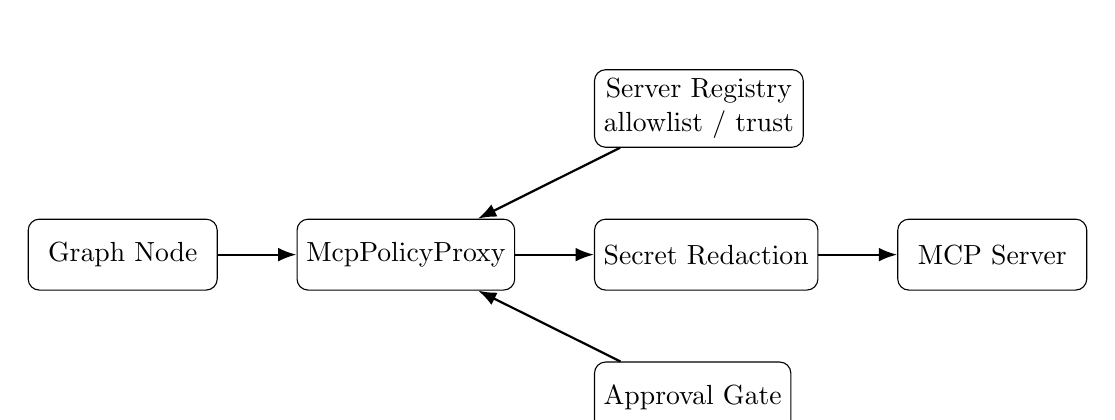
\begin{tikzpicture}[
  node distance=9mm and 10mm,
  box/.style={draw, rounded corners, align=center, minimum width=24mm, minimum height=9mm},
  flow/.style={-Latex, thick}
]
\node[box] (graph) {Graph Node};
\node[box, right=of graph] (proxy) {McpPolicyProxy};
\node[box, above right=of proxy] (registry) {Server Registry\\allowlist / trust};
\node[box, below right=of proxy] (approval) {Approval Gate};
\node[box, right=of proxy] (redact) {Secret Redaction};
\node[box, right=of redact] (server) {MCP Server};

\draw[flow] (graph) -- (proxy);
\draw[flow] (registry) -- (proxy);
\draw[flow] (approval) -- (proxy);
\draw[flow] (proxy) -- (redact);
\draw[flow] (redact) -- (server);
\end{tikzpicture}

\end{center}

\begin{qaBox}{固定表述}
MCP 是协议，不是治理系统。真正安全的接法不是把 MCP Tool 直接映射成 LangChain Tool，而是先过 \term{McpPolicyProxy}，把 server allowlist、tool allowlist、只读默认和 secret redaction 做成强闸门。
\end{qaBox}

\subsection{五类幻觉怎么治理}
\begin{itemize}[leftmargin=2em]
  \item 知识幻觉：先检索，证据不足就拒答，不能拿模型记忆补业务事实。
  \item 工具幻觉：Observation 必须来自真实工具返回，不能让模型伪造 tool result。
  \item 参数幻觉：schema 校验不过就不执行，工具调用是接口，不是聊天。
  \item 证据幻觉：分析和报告必须能回溯到证据和 citation。
  \item 行动幻觉：高风险工具默认不执行，需要动作级审批门。
\end{itemize}

\section{第九轮拷打：高压追问怎么接}

\begin{summaryBox}{这一轮面试官在试什么}
到这一轮，面试官往往已经默认你做过一些东西了。他接下来要看的是：当问题被压得很细、很尖锐时，你能不能既守住事实边界，又把架构判断讲透。下面这些问题适合直接背熟成口头版。
\end{summaryBox}

\subsection{为什么选择 LangGraph，而不是直接做多 Agent 对话}
\begin{qaBox}{答案}
多 Agent 对话更适合开放式协作，不适合强流程研究任务。研究任务要求节点、依赖、预算、审计和恢复都可显式表达，LangGraph 这种状态机编排比纯消息流更适合工程化落地。
\end{qaBox}

\subsection{为什么动作审批的权威源必须是 DB}
\begin{qaBox}{答案}
因为动作执行是高风险事实，不能依赖多个远端状态拼凑出来。数据库里的审批聚合根必须是唯一裁决者，否则系统会出现“远端已批、本地未落”“远端已拒、本地重试继续跑”这类危险分叉。
\end{qaBox}

\subsection{为什么外部审批不能直接作为执行依据}
\begin{qaBox}{答案}
外部审批更适合作为输入信号，不适合作为最终执行前判定。标准做法是外部系统回调统一落库，更新本地审批状态，再由本地状态决定是否允许动作执行。这样幂等、审计和重试逻辑才有单一依赖点。
\end{qaBox}

\subsection{为什么要在 LangGraph 外再加 Harness}
\begin{qaBox}{答案}
因为如果把失败恢复、预算熔断、审批暂停、worker 抢租约和任务恢复都塞进图里，图就会从“业务工作流”膨胀成“超级控制器”。Harness 的价值在于把任务级控制面从业务级编排面剥离出去。
\end{qaBox}

\subsection{为什么 MCP 必须先过 policy proxy}
\begin{qaBox}{答案}
因为 MCP 只定义了如何暴露工具，不定义工具是否可信、参数是否越权、结果是否含敏感信息、危险写操作是否需要审批。没有 policy proxy，MCP 接入越多，系统越接近裸奔。
\end{qaBox}

\subsection{预算治理为什么不能只做软提示}
\begin{qaBox}{答案}
软提示只能告诉你“快超了”，不能真正止损。对长任务 Agent 来说，真正需要的是硬熔断加优雅降级：达到阈值后停止可选工具节点，禁止进一步 replan，最后基于当前证据输出部分报告。这才叫治理，不叫提醒。
\end{qaBox}

\section{附录：当前仓库现实、边界与演进路线}

\begin{summaryBox}{附录怎么用}
附录不是给面试官从头念的，而是给你自己在面试前校准边界。只要这里写的是“未完成”，面试时就不要包装成“已经具备”。只要这里写的是“设计已定”，面试时就要明确补一句“但代码尚未完整接入”。
\end{summaryBox}

\subsection{当前已核实的现实结论}
\begin{itemize}[leftmargin=2em]
  \item 聚合器覆盖失败语义的历史 bug 已经修复，不应继续当作现存问题对外表述。
  \item \term{tool\_call\_audit} 已落地，工具审计不再只依赖 session JSON。
  \item \term{session\_budget\_state} 已落地，预算状态开始从 \term{review\_status} 中拆出。
  \item session 级 breaker 已有最小可用版，但 token/cost 精度仍未完全做满。
  \item 动作级审批尚未真正接入执行流。
  \item MCP 仍未实际接入；如果未来直接接入而不加 proxy，风险非常高。
\end{itemize}

\subsection{当前仍存在的关键边界}
\begin{riskBox}{需要诚实面对的点}
第一，审批仍主要停留在任务入口，不是动作级审批。第二，tool audit 和 budget state 目前以 workflow 收尾持久化为主，仍非 crash-safe。第三，Harness supervisor 设计已明确，但还没形成完整外层恢复控制。第四，MCP policy proxy 仍未落地。
\end{riskBox}

\subsection{建议的三阶段演进}
\begin{enumerate}[leftmargin=2em]
  \item Phase 1：失败语义显式化、tool audit 持久化、会话级 budget breaker、session budget state。
  \item Phase 2：Harness supervisor、batch boundary checkpoint、任务级恢复与租约。
  \item Phase 3：动作级审批、MCP policy proxy、外部审批系统信号接入。
\end{enumerate}

\subsection{最终的面试总结句}
\begin{qaBox}{收口}
如果只看主链路，这个项目已经是一个能工作的研究型 Agent。真正让我认为它有工程价值的地方，在于它没有停留在“会规划、会搜索、会写报告”这一步，而是开始把失败语义、预算、审计、审批和外部工具边界都纳入系统设计。也正因为如此，它既能讲 Agent 能力，也能讲 Agent 治理。
\end{qaBox}

\end{document}
